\documentclass{beamer}

%style
\mode<presentation>{
	\usetheme{goettingen}
}
%packages
\usepackage[utf8]{inputenc}
\usepackage[ngerman]{babel}
\usepackage{graphicx}
\usepackage{tikz}

%Einstellungen Präsentation
\title{Gabor Wavelets und Visuelle Wahrnehmung}
\author{Raphael Unterer}
\institute{Mathematisches Seminar 2018}
\date{27.05.2019}

%Bilder
\graphicspath{{images/}}

%Beginn der Präsentation
\begin{document}

%Titelseite
\begin{frame}
\titlepage
\end{frame}

%Inhaltsverzeichnis
%\begin{frame}
%\frametitle{Inhalt}
%\tableofcontents
%\end{frame}

\section{Gabor Wavelets}

\begin{frame}
	\frametitle{Repetition Gabor-Wavelets}
	\begin{itemize}
		\item[] Exponentiell abfallende komplexe Exponenten (Sinus und Kosinus)
		\begin{figure}
			\centering
			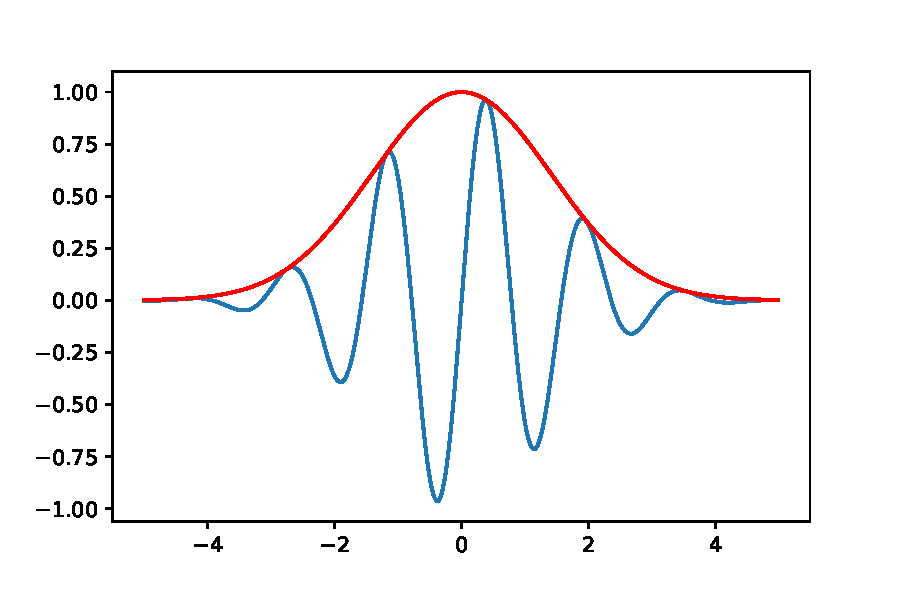
\includegraphics[width=0.7\linewidth]{images/gabor_1d}
			\caption{Sinus Gabor Wavelet 1D}
			\label{fig:gabor1d}
		\end{figure}
	\end{itemize}
\end{frame}

\begin{frame}
	\frametitle{2D Gabor Wavelets}
	\begin{itemize}
		\item[]
		\begin{equation}
			G(x,y)=\frac{1}{2\pi\sigma\beta}
			e^{-\pi(\frac{(x-x_{0})^{2}}{\sigma^{2}}+\frac{(y-y_{0})^{2}}{\beta^{2}})}
			e^{i(\xi_{0}x+\nu_{0}y)}
		\end{equation}
		\pause
		\item[] Praktischer:
		\begin{equation}
			G(x,y)=e^{-\frac{x'^{2}+\gamma^{2}y'^{2}}{2\sigma^{2}}}
			e^{i(2\pi\frac{x'}{\lambda} + \phi)}
		\end{equation}
		\pause
		\item[] mit:
		\begin{equation}
		x'=x\cos(\theta)+y\sin(\theta)
		\end{equation}
		\item[] und:
		\begin{equation}
		y'=-x\sin(\theta)+y\cos(\theta)
		\end{equation}
			
	\end{itemize}
\end{frame}

\begin{frame}
\frametitle{2D Gabor Wavelets}
	\begin{figure}
		\centering
		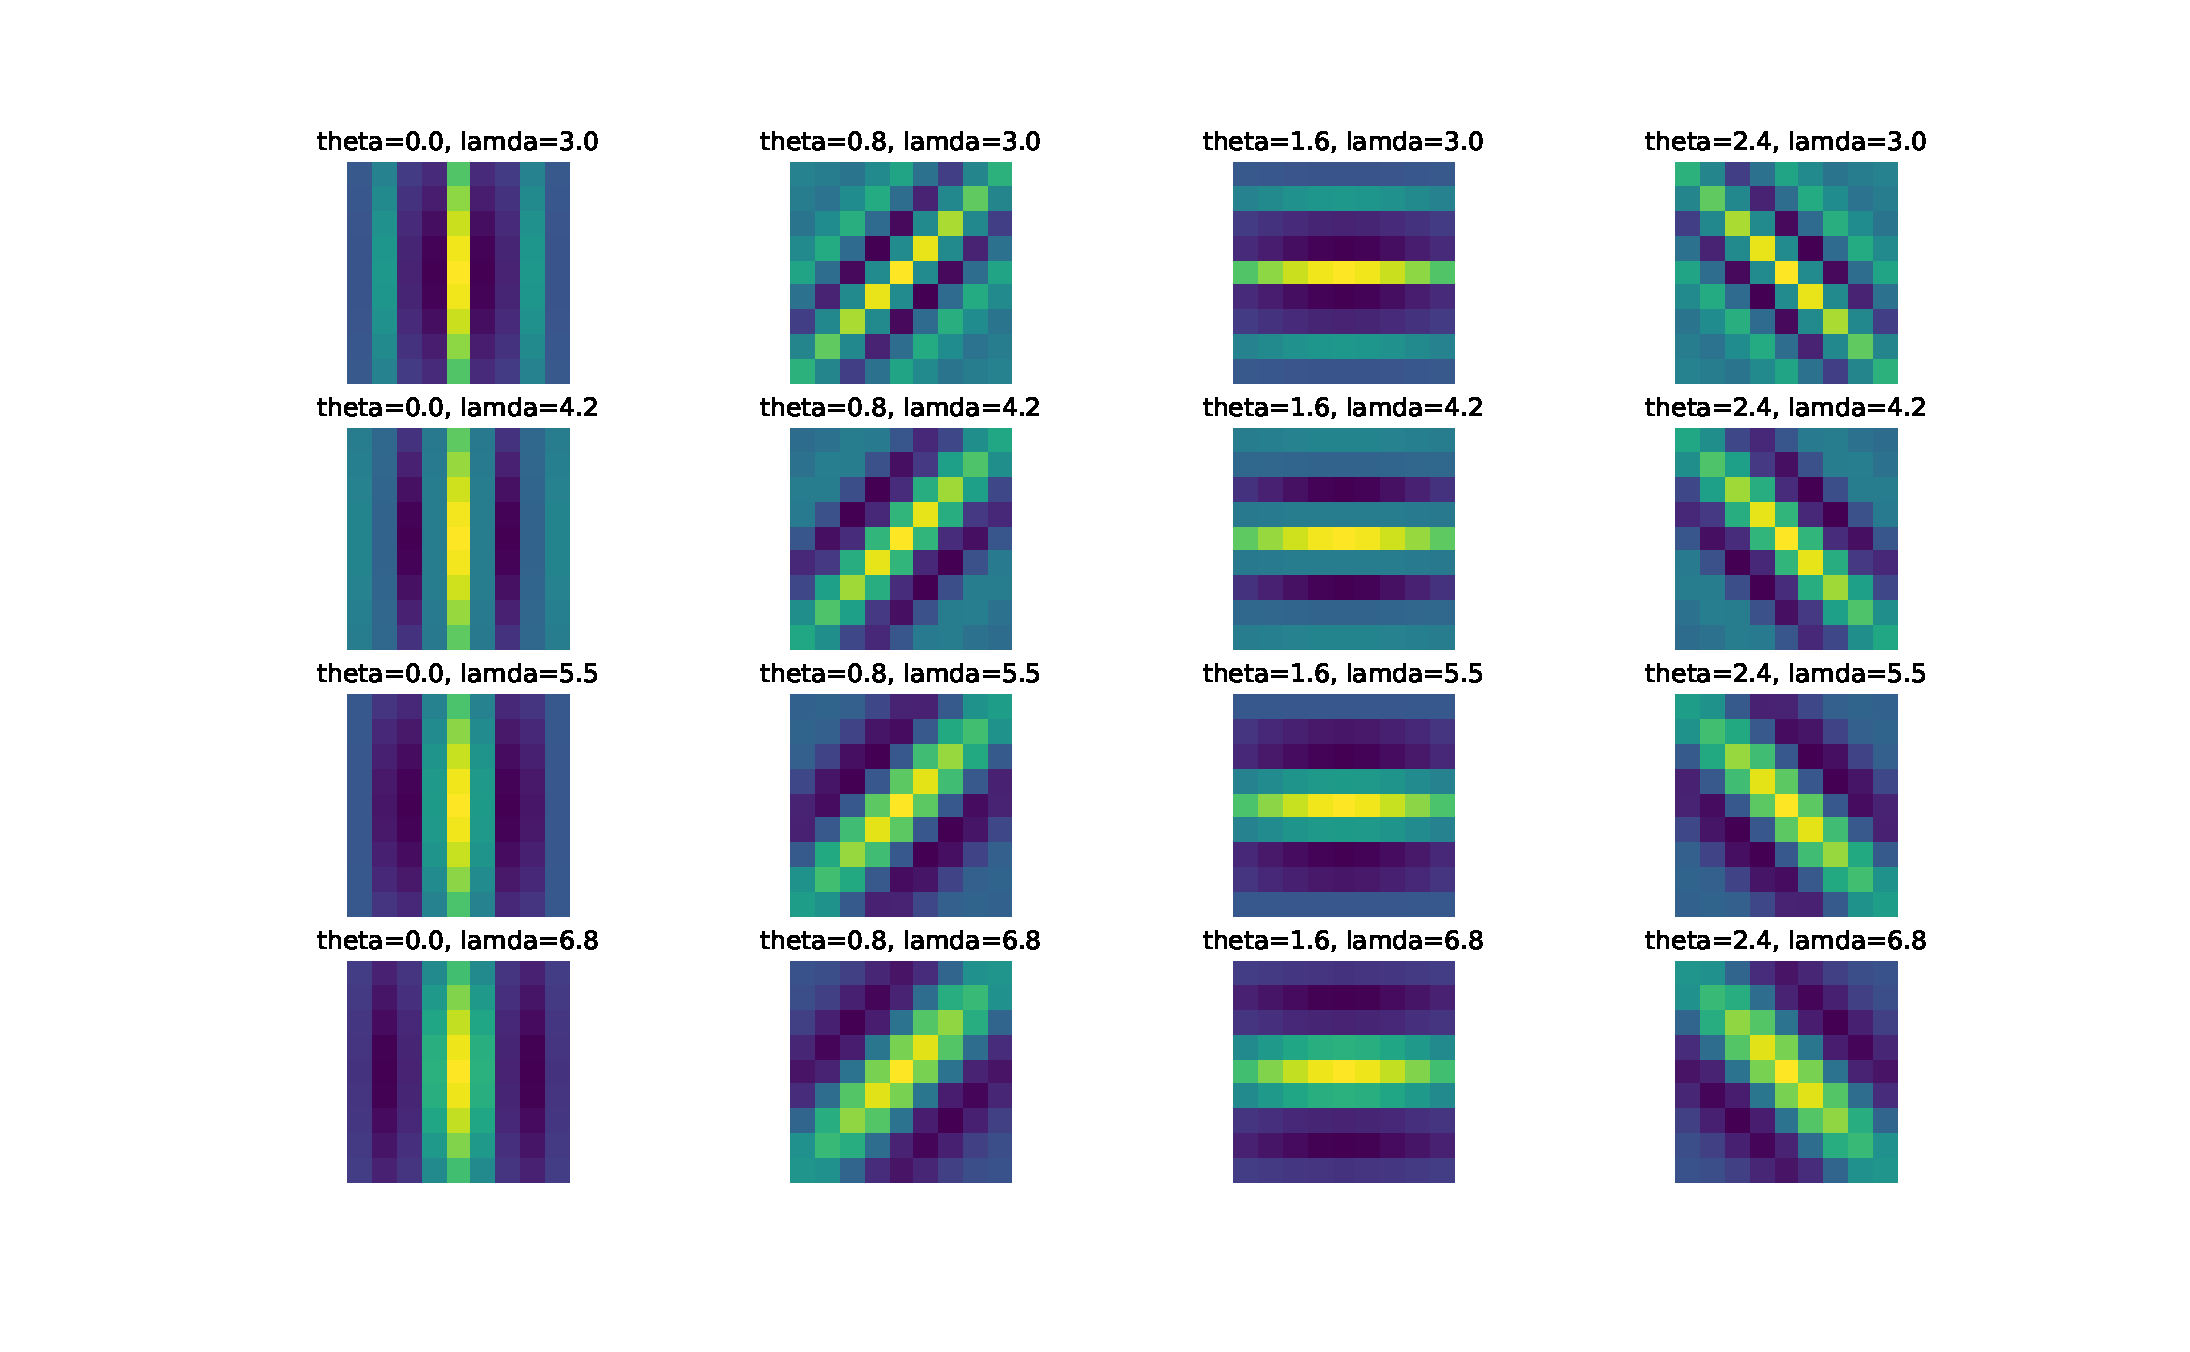
\includegraphics[width=\linewidth]{images/gabor_2d}
		\caption{Theta $\theta$ und Wellenlänge $\lambda$ ändern}
		\label{fig:gabor2d}
	\end{figure}	

\end{frame}

\begin{frame}
\frametitle{2D Gabor Wavelets}
\begin{figure}
	\centering
	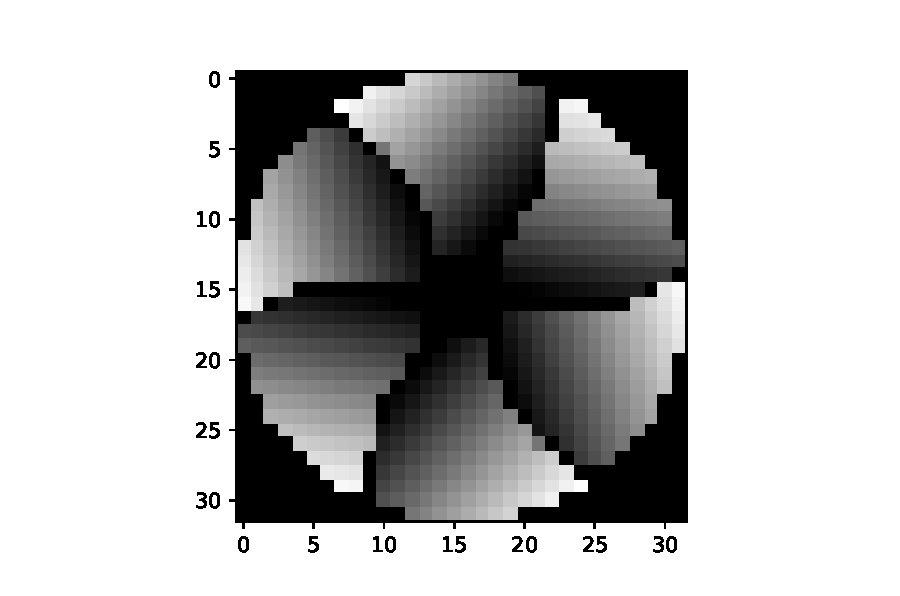
\includegraphics[width=\linewidth]{images/gabor_effect_original.pdf}
	\caption{Beispielbild}
	\label{fig:gabororiginal}
\end{figure}	
\end{frame}

\begin{frame}
\frametitle{2D Gabor Wavelets}
\begin{figure}
	\centering
	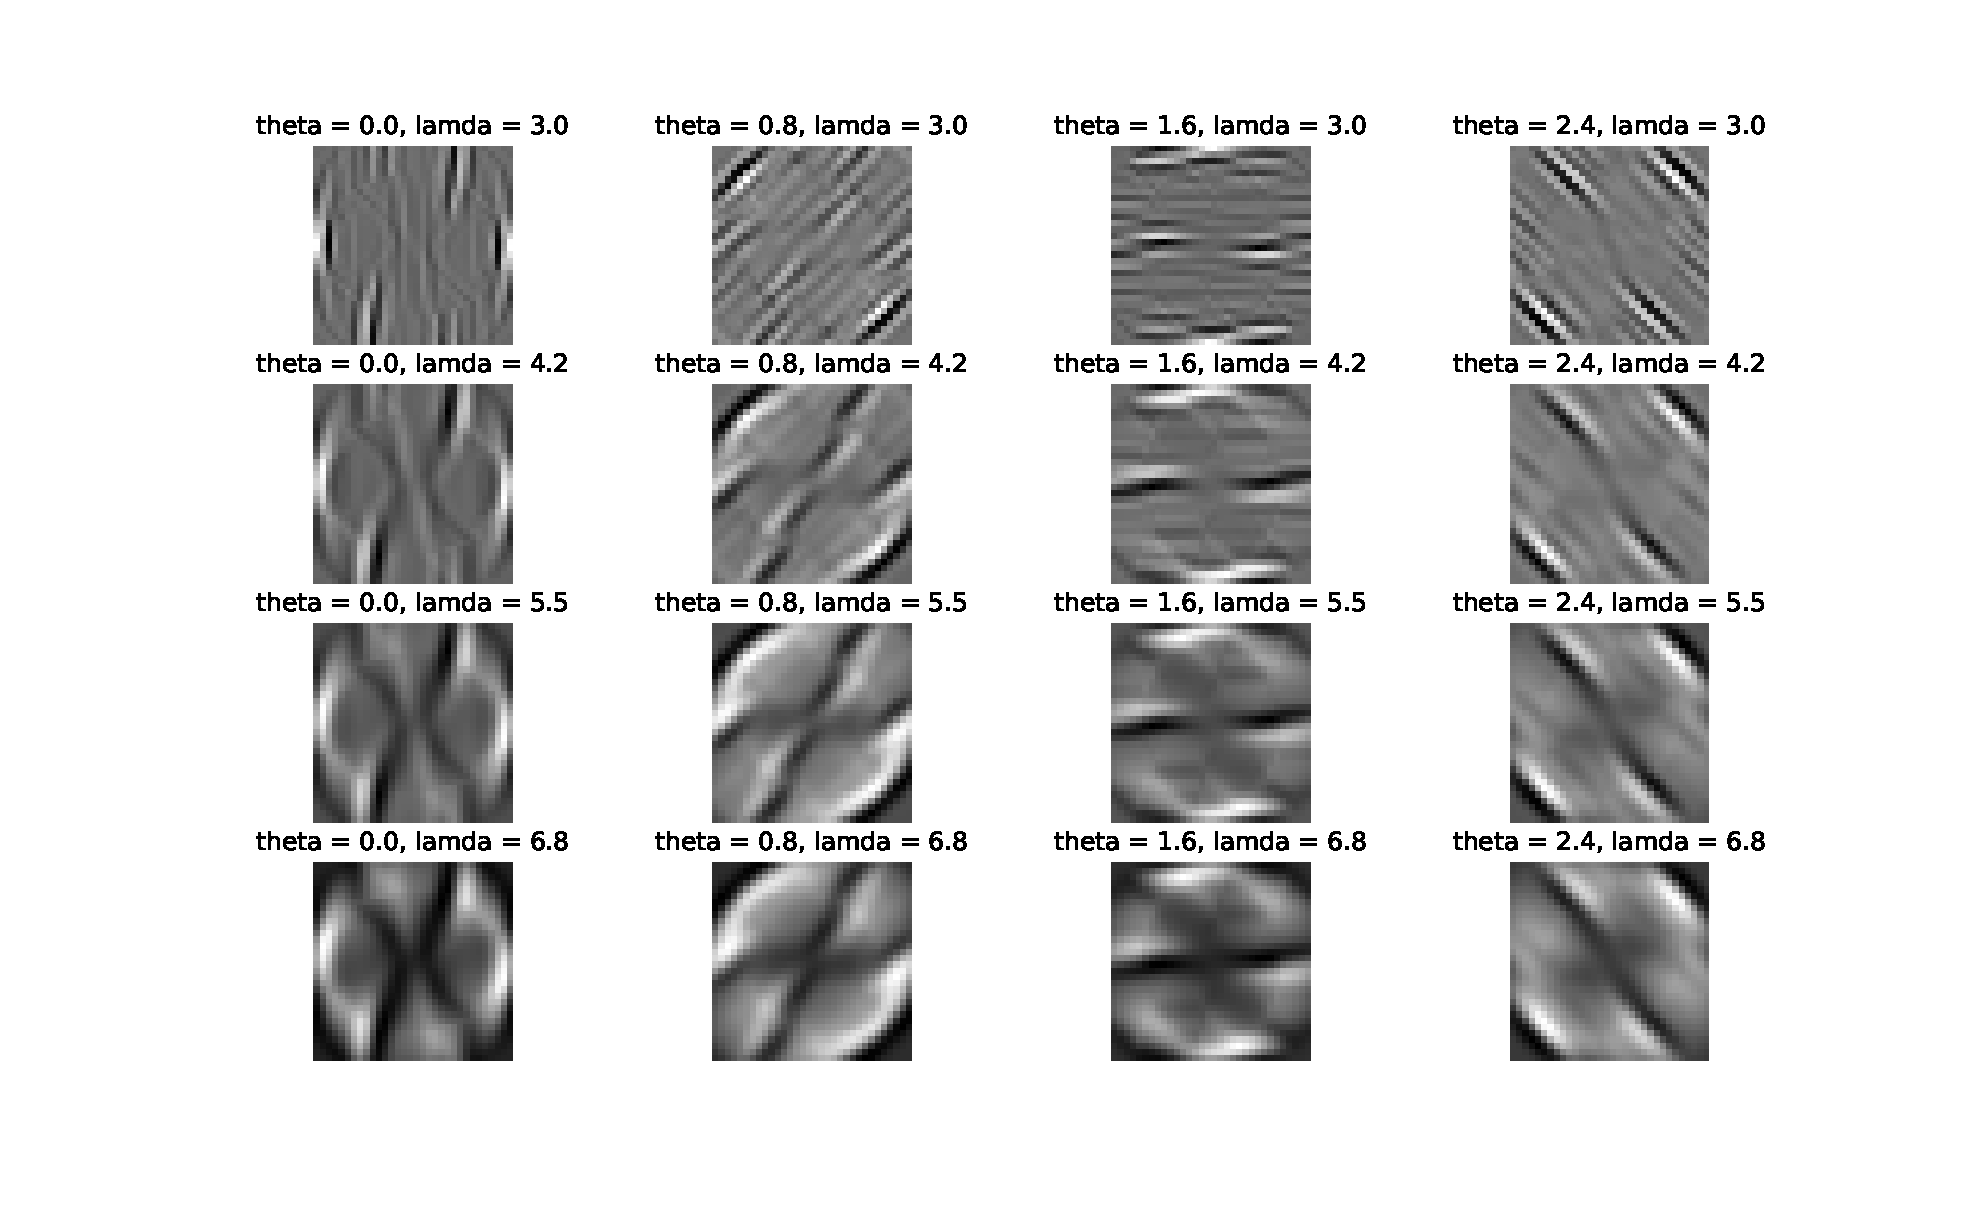
\includegraphics[width=\linewidth]{images/gabor_effect_effect.pdf}
	\caption{Gabor-Filter angewandt auf das Beispielbild}
	\label{fig:gaboreffect}
\end{figure}	

\end{frame}

\begin{frame}
\frametitle{2D Wavelet Transformation als 2D Convolution}
\usetikzlibrary{matrix, positioning}
\begin{tikzpicture}

	\matrix (mtr) [matrix of nodes,row sep=-\pgflinewidth, nodes={draw}]
	{
		0 & 1 & 1 & |[fill=red!30]| 1 & |[fill=red!30]| 0 & |[fill=red!30]| 0 & 0\\
		0 & 0 & 1 & |[fill=red!30]| 1 & |[fill=red!30]| 1 & |[fill=red!30]| 0 & 0\\
		0 & 0 & 0 & |[fill=red!30]| 1 & |[fill=red!30]| 1 & |[fill=red!30]| 1 & 0\\
		0 & 0 & 0 & 1 & 1 & 0 & 0\\
		0 & 0 & 1 & 1 & 0 & 0 & 0\\
		0 & 1 & 1 & 0 & 0 & 0 & 0\\
		1 & 1 & 0 & 0 & 0 & 0 & 0\\
	};

	\draw[very thick, red] (mtr-1-4.north west) rectangle (mtr-3-6.south east);

	\node [below= of mtr-5-4.south] (lm) {$\bf I$};

	\node[right = 0.2em of mtr] (str) {$*$};

	\matrix (K) [right=0.2em of str,matrix of nodes,row sep=-\pgflinewidth, nodes={draw, fill=blue!30}]
	{
		1 & 0 & 1 \\
		0 & 1 & 0 \\
		1 & 0 & 1 \\
	};
	\node [below = of K-3-2.south] (lk) {$\bf K$};

	\node [right = 0.2em of K] (eq) {$=$};

	\matrix (ret) [right=0.2em of eq,matrix of nodes,row sep=-\pgflinewidth, nodes={draw}]
	{
		1 & 4 & 3 & |[fill=green!30]| 4 & 1\\
		1 & 2 & 4 & 3 & 3\\
		1 & 2 & 3 & 4 & 1\\
		1 & 3 & 3 & 1 & 1\\
		3 & 3 & 1 & 1 & 0\\
	};
	\node [below = of ret-4-3.south] (lim) {${\bf I} * {\bf K}$};

	\draw[very thick, green] (ret-1-4.north west) rectangle (ret-1-4.south east);

	\draw[densely dotted, blue, thick] (mtr-1-4.north west) -- (K-1-1.north west);
	\draw[densely dotted, blue, thick] (mtr-3-4.south west) -- (K-3-1.south west);
	\draw[densely dotted, blue, thick] (mtr-1-6.north east) -- (K-1-3.north east);
	\draw[densely dotted, blue, thick] (mtr-3-6.south east) -- (K-3-3.south east);

	\draw[densely dotted, green, thick] (ret-1-4.north west) -- (K-1-1.north west);
	\draw[densely dotted, green, thick] (ret-1-4.south west) -- (K-3-1.south west);
	\draw[densely dotted, green, thick] (ret-1-4.north east) -- (K-1-3.north east);
	\draw[densely dotted, green, thick] (ret-1-4.south east) -- (K-3-3.south east);

	\matrix (K) [right=0.2em of str,matrix of nodes,row sep=-\pgflinewidth, nodes={draw, fill=blue!10}]
	{
		1 & 0 & 1 \\
		0 & 1 & 0 \\
		1 & 0 & 1 \\
	};

	\draw[very thick, blue] (K-1-1.north west) rectangle (K-3-3.south east);

	\node[anchor=south east, inner sep=0.01em, blue] at (mtr-1-4.south east) (xx) {\scalebox{.5}{$\times 1$}};
	\node[anchor=south east, inner sep=0.01em, blue] at (mtr-1-5.south east) (xx) {\scalebox{.5}{$\times 0$}};
	\node[anchor=south east, inner sep=0.01em, blue] at (mtr-1-6.south east) (xx) {\scalebox{.5}{$\times 1$}};
	\node[anchor=south east, inner sep=0.01em, blue] at (mtr-2-4.south east) (xx) {\scalebox{.5}{$\times 0$}};
	\node[anchor=south east, inner sep=0.01em, blue] at (mtr-2-5.south east) (xx) {\scalebox{.5}{$\times 1$}};
	\node[anchor=south east, inner sep=0.01em, blue] at (mtr-2-6.south east) (xx) {\scalebox{.5}{$\times 0$}};
	\node[anchor=south east, inner sep=0.01em, blue] at (mtr-3-4.south east) (xx) {\scalebox{.5}{$\times 1$}};
	\node[anchor=south east, inner sep=0.01em, blue] at (mtr-3-5.south east) (xx) {\scalebox{.5}{$\times 0$}};
	\node[anchor=south east, inner sep=0.01em, blue] at (mtr-3-6.south east) (xx) {\scalebox{.5}{$\times 1$}};

\end{tikzpicture}
\end{frame}


\begin{frame}
	\frametitle{Neurologie}
	\begin{figure}
		\centering
		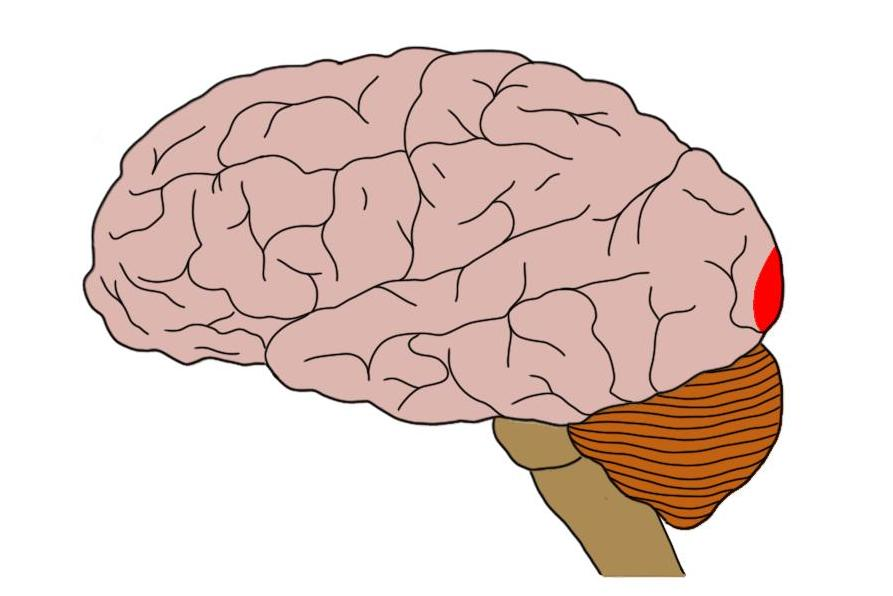
\includegraphics[width=0.7\linewidth]{primary-visual-cortex.jpg}
		\caption{Primärer Visueller Kortex in rot}
		\label{fig:primary-visual-cortex}
	\end{figure}
	
\end{frame}

\section{Convolutional Neural Net (CNN)}
\begin{frame}
\frametitle{Neuronale Netze}
\begin{figure}
	\centering
	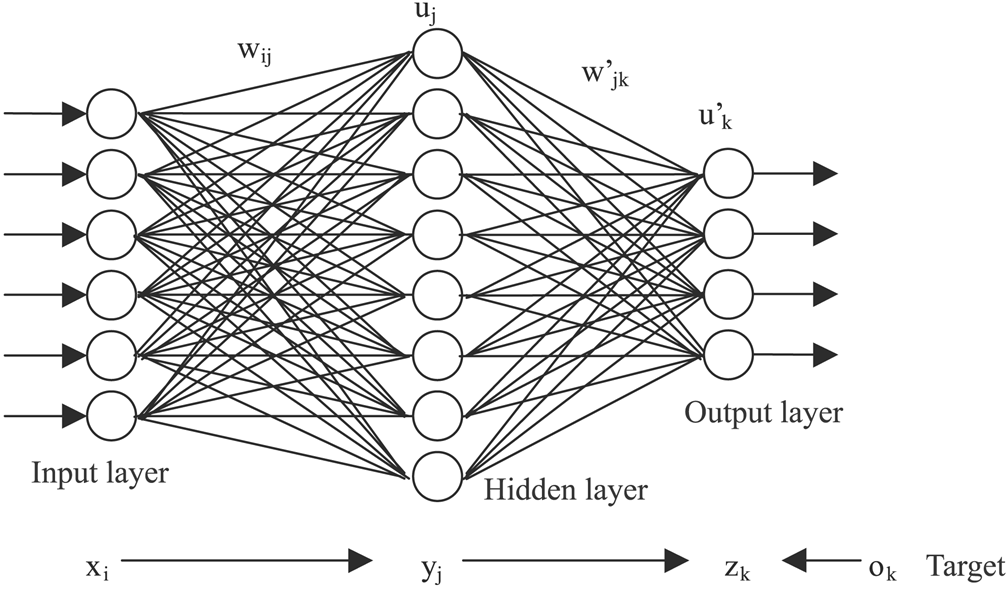
\includegraphics[width=0.7\linewidth]{neural_net}
	\caption{Schematische Darstellung eines Neuronalen Netzes}
	\label{fig:neuralnet}
\end{figure}

\end{frame}

\begin{frame}
\frametitle{CIFAR-10 Dataset}
	\begin{figure}
		\centering
		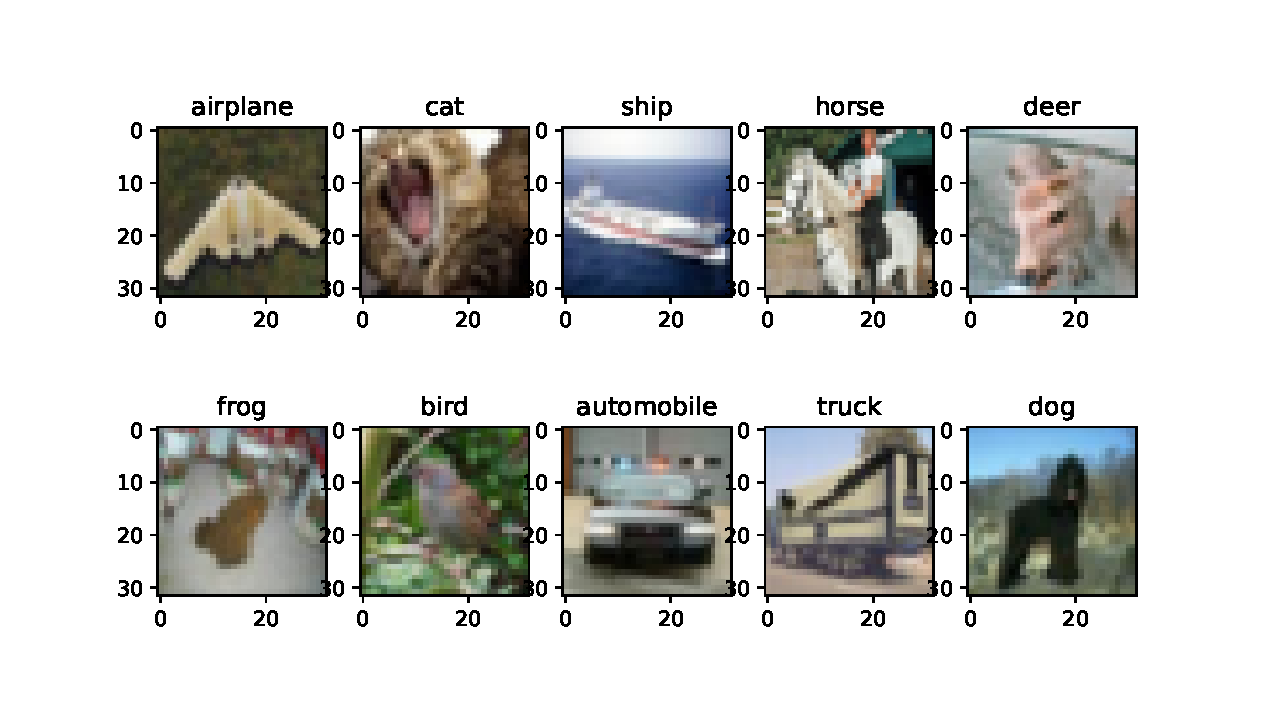
\includegraphics[width=\linewidth]{images/cifar10}
		\label{fig:cifar10}
	\end{figure}
	
\end{frame}


\begin{frame}
\frametitle{Architektur}
\begin{figure}
	\centering
	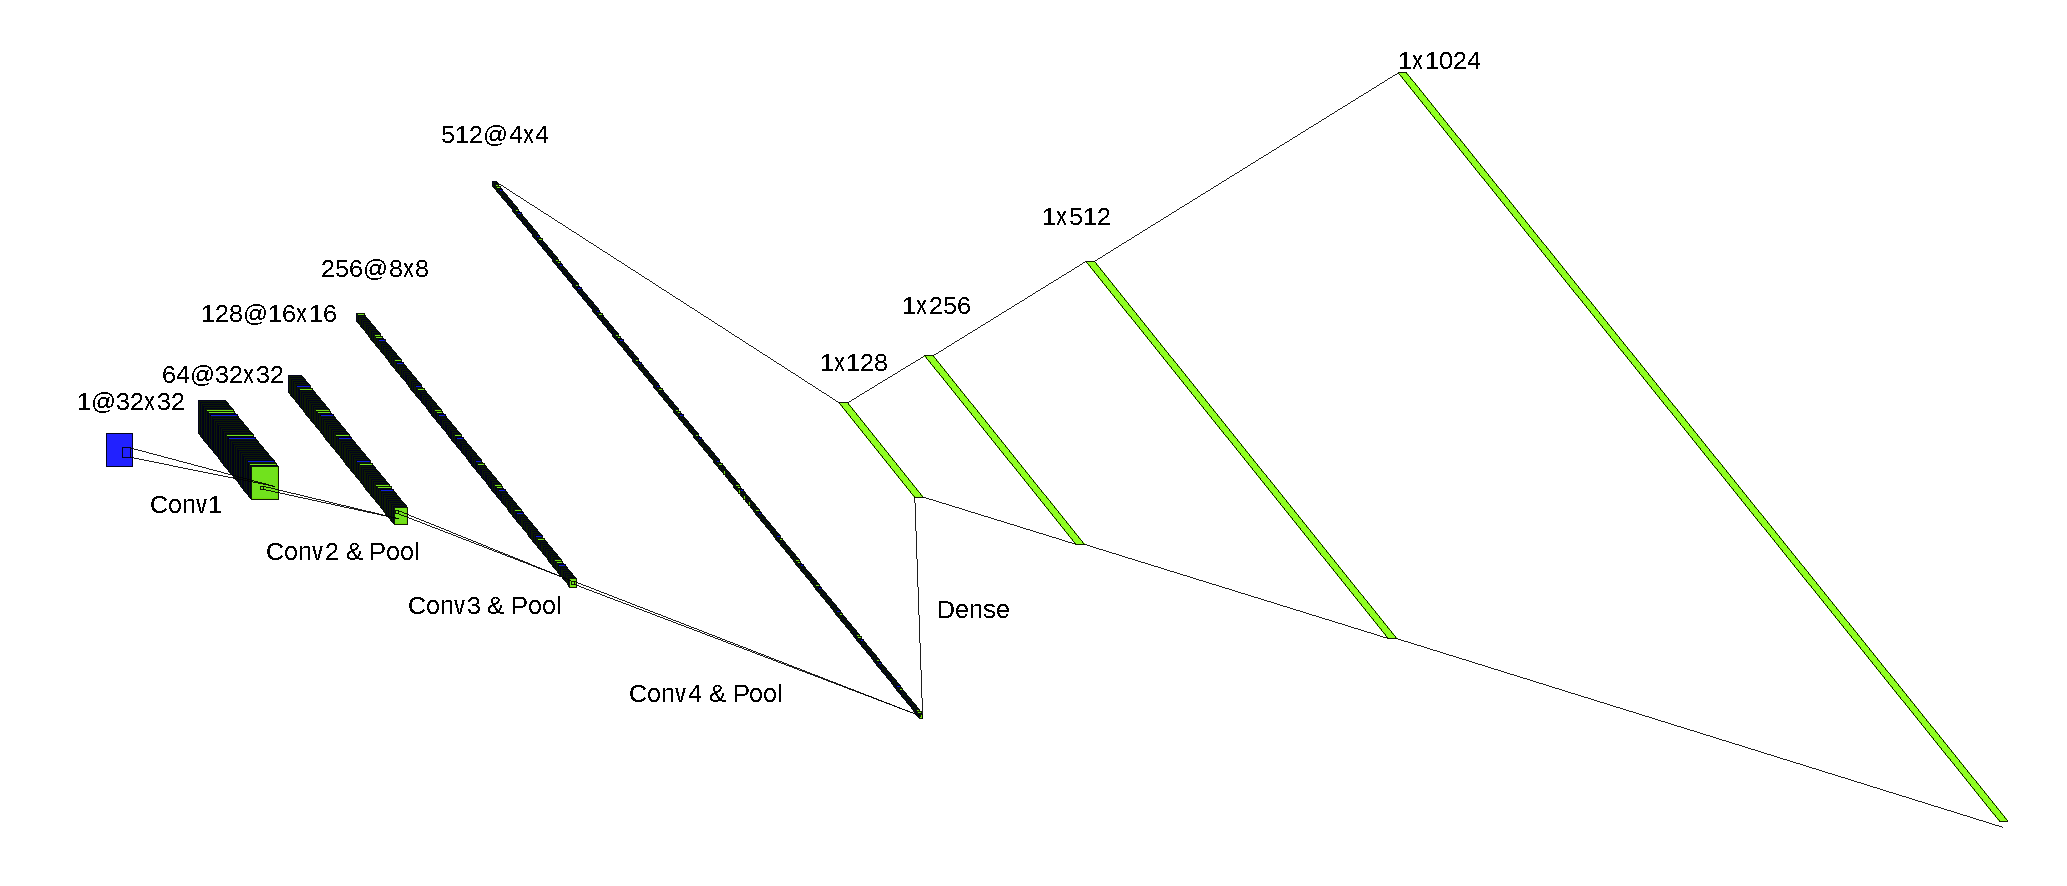
\includegraphics[width=\linewidth]{cnn.pdf}
	\label{fig:cnn}
\end{figure}
\begin{itemize}
	\item[] First convolutional layer: 64 9x9 kernels
\end{itemize}

\end{frame}


\begin{frame}
\frametitle{Experiment}
	\begin{itemize}
		 \item [] Erste Convolution mit Gabor-Kernels durchgeführt:
	\end{itemize}
	\begin{figure}
		\centering
		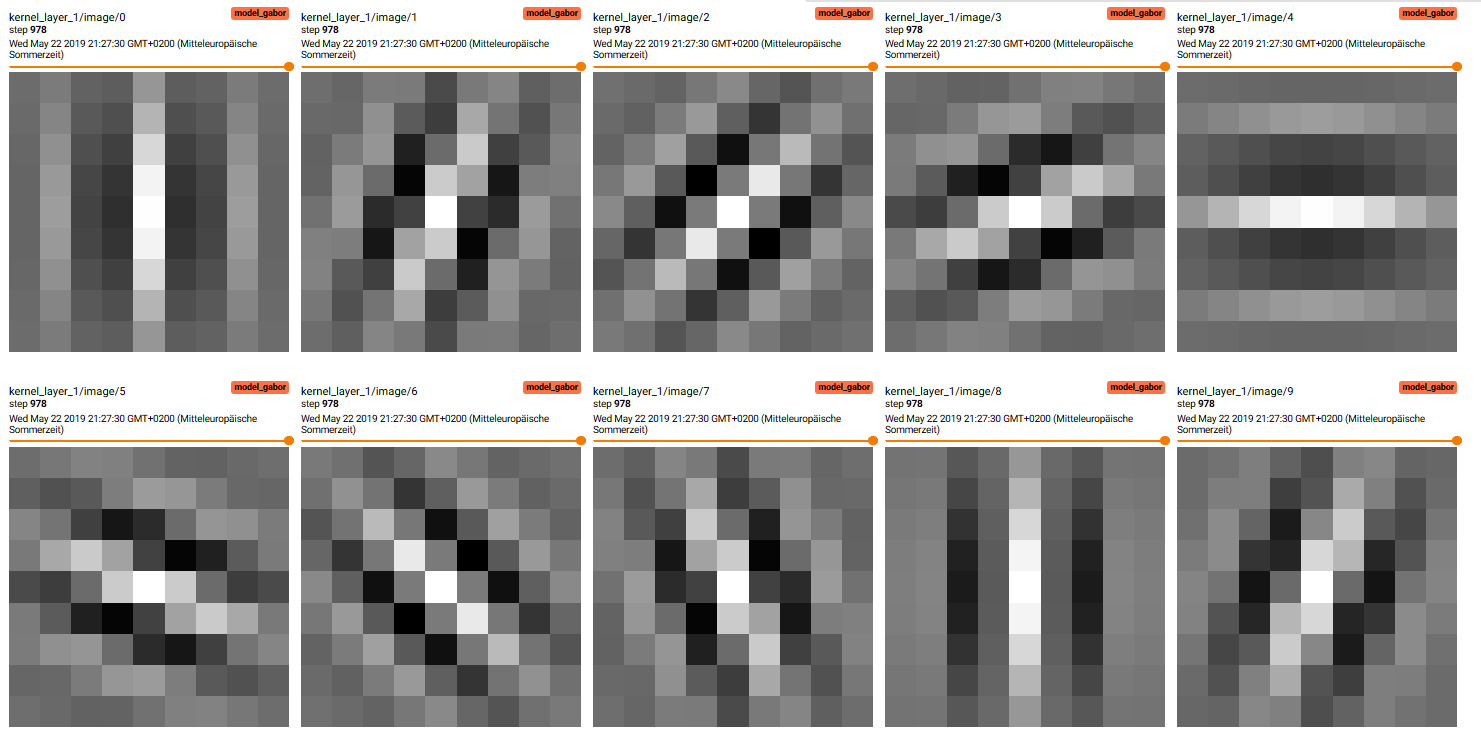
\includegraphics[width=\linewidth]{images/gabor_kernels}
		\label{fig:gaborkernels}
	\end{figure}
	
\end{frame}


\section{Resultate}

\begin{frame}
\frametitle{Performance}
\begin{itemize}
	\item[] Kleinste Accuracy mit Gabor: 67.32\%
	\item[] Höchste Accuracy ohne Gabor: 66.42\%
\end{itemize}
\begin{figure}
	\centering
	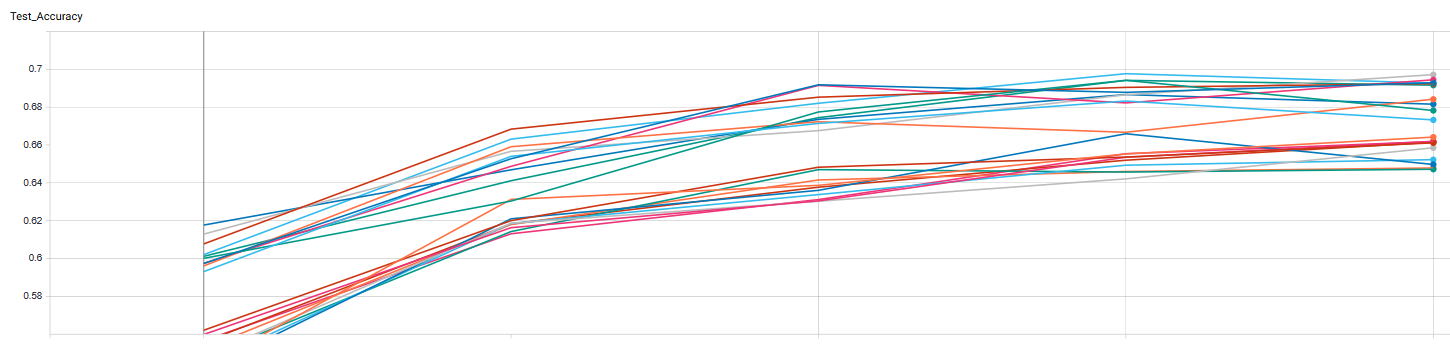
\includegraphics[width=\linewidth]{comparison.png}
	\label{fig:comparison}
\end{figure}

\end{frame}

\begin{frame}
\frametitle{Gelernte Filter}
\begin{figure}
	\centering
	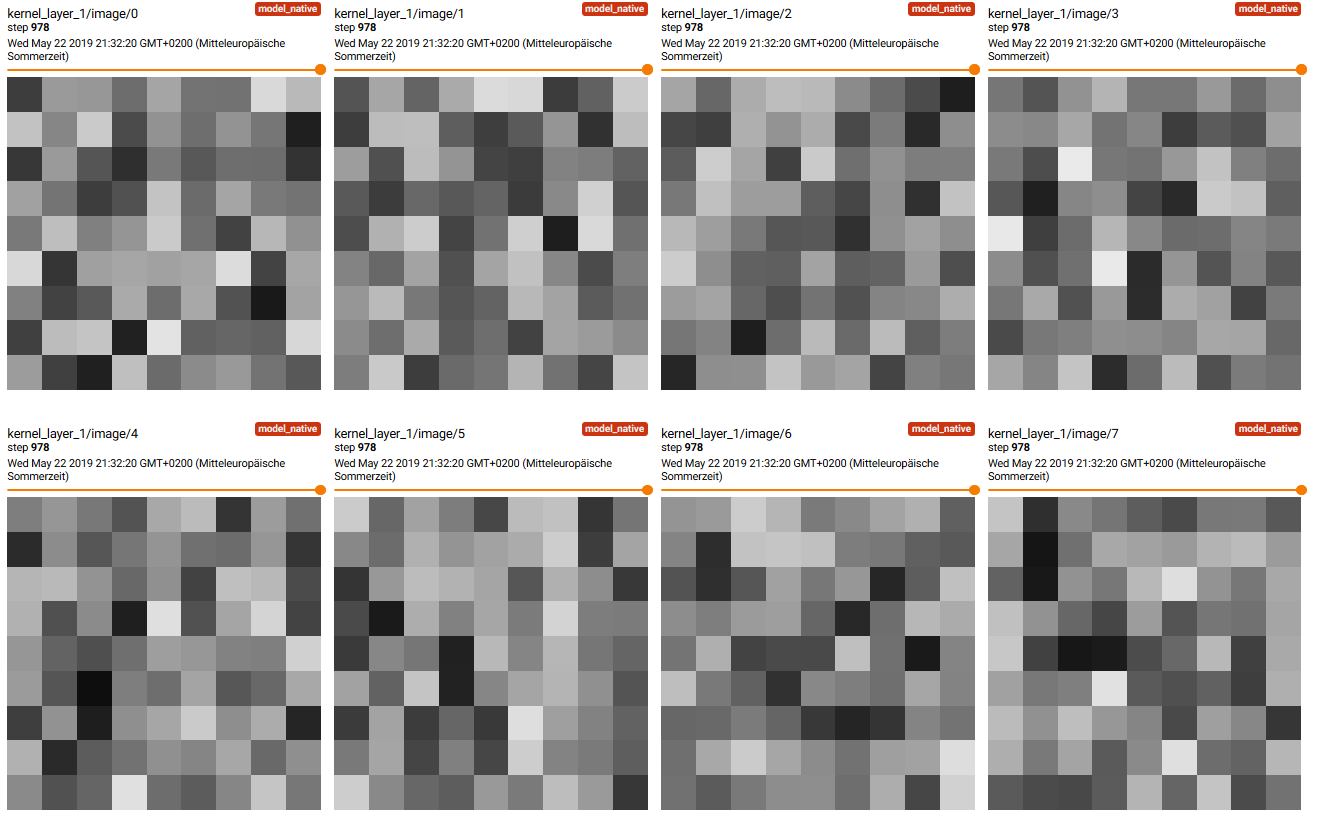
\includegraphics[width=\linewidth]{images/native_kernels}
	\label{fig:nativekernels}
\end{figure}
\end{frame}

\begin{frame}
\frametitle{Ende}
\end{frame}
\end{document}